\chapter{Numerical Methods for Non-Hermitian Maxwell Problems}
\label{ch:numerics}

\begin{chapterlead}
The analytical methods developed in previous chapters---coupled-mode
theory, transfer matrices, perturbative expansions---reach their limits
when the geometry is complex, the non-Hermiticity is strong, or many
modes interact. Numerical methods are then essential. This chapter
develops the principal computational approaches to non-Hermitian photonic
problems in depth: the finite-element method with perfectly matched
layers, plane-wave expansion for complex band structures, time-domain
simulation of gain/loss media, and specialized algorithms for
quasinormal-mode extraction, exceptional-point tracking, and non-Bloch
invariant computation. The emphasis throughout is on what changes when
Hermiticity is lost, where standard numerical photonics tools need
modification, and how to validate results in a setting where intuition
from Hermitian spectral theory no longer applies.
\end{chapterlead}


%% ================================================================
\section{The computational workflow}
\label{sec:workflow}

Before describing individual methods, it is useful to outline the
typical workflow for a non-Hermitian Maxwell computation. The steps
are:
\begin{enumerate}
 \item \textbf{Geometry and material definition.} Specify the spatial
 distribution of $\epsr(\rr,\omega)$ and $\mur(\rr,\omega)$,
 including complex (lossy/gain) and frequency-dispersive components.
 \item \textbf{Boundary treatment.} For open systems, surround the
 scatterer with a perfectly matched layer (PML) or impose
 transparent/radiation boundary conditions.
 \item \textbf{Discretization.} Convert the continuous Maxwell
 operator into a finite-dimensional matrix problem using FEM, PWE,
 or FDTD.
 \item \textbf{Eigenvalue extraction.} Find the complex
 eigenfrequencies $\omtil_n$ using a non-Hermitian eigensolver
 (shift-and-invert Arnoldi, contour-integral method, or
 Newton-type pole search).
 \item \textbf{Adjoint modes and normalization.} Compute the left
 eigenvectors (adjoint modes) and normalize using the unconjugated
 biorthogonal prescription of Section~\ref{sec:qnm-normalization}.
 \item \textbf{Post-processing.} Reconstruct physical observables
 (scattering spectra, LDOS, Purcell factors, topological invariants)
 from the modal expansion.
 \item \textbf{Validation.} Verify that QNM eigenfrequencies are
 independent of PML parameters, cross-check between methods, and
 assess convergence.
\end{enumerate}

Each step introduces challenges specific to non-Hermitian systems that
we now discuss in detail.


%% ================================================================
\section{Finite-element method with PML}
\label{sec:fem-pml}

The finite-element method (FEM) discretizes the Maxwell equations on an
unstructured mesh, making it well suited to complex geometries. For
open systems, PML (Section~\ref{sec:pml}) truncates the computational
domain and converts the problem into a finite-dimensional non-Hermitian
generalized eigenvalue problem~\cite{vial2014quasimodal}.

\subsection{Weak formulation of the Maxwell eigenproblem}
\label{ssec:weak-form}

The frequency-domain Maxwell curl-curl equation for the electric field,
\begin{equation}
 \curl\!\left[\mur^{-1}\curl\EE\right]
 = \frac{\omega^2}{c^2}\,\epsr(\omega)\,\EE,
 \label{eq:curl-curl-e}
\end{equation}
is converted to weak form by multiplying by a test function
$\mathbf{F}$ and integrating over the computational domain $\Omega$
(including the PML region):
\begin{equation}
 \int_\Omega (\curl\mathbf{F})\cdot\mur^{-1}\curl\EE\;\dd V
 = \frac{\omega^2}{c^2}\int_\Omega
 \mathbf{F}\cdot\epsr(\omega)\,\EE\;\dd V.
 \label{eq:weak-form}
\end{equation}
After FEM discretization with N\'ed\'elec (edge) elements, this becomes
the generalized eigenvalue problem
\begin{equation}
 \mathbf{A}\,\mathbf{x} = \omtil^2\,\mathbf{B}\,\mathbf{x},
 \label{eq:fem-gep}
\end{equation}
where $\mathbf{A}$ encodes the curl--curl operator and boundary terms,
$\mathbf{B}$ encodes the material weight $\epsr/c^2$ (including PML
stretching), and $\omtil$ is the complex eigenfrequency.

\subsection{PML implementation}
\label{ssec:pml-implementation}

The PML is implemented by the complex coordinate
stretching~\eqref{eq:pml-stretch}, which modifies the material tensors
in the PML region. In three dimensions, the stretching is applied
independently in each Cartesian direction through a diagonal tensor
$\boldsymbol{\Lambda}$:
\begin{equation}
 \boldsymbol{\Lambda} = \mathrm{diag}
 \left(\frac{s_y s_z}{s_x},\;
 \frac{s_x s_z}{s_y},\;
 \frac{s_x s_y}{s_z}\right),
 \label{eq:pml-tensor}
\end{equation}
where $s_\alpha = 1 + i\sigma_\alpha(\alpha)/\omega$ is the stretching
factor in direction $\alpha$. The PML-modified permittivity and
permeability are
$\epsr^{\mathrm{PML}} = \boldsymbol{\Lambda}\,\epsr$ and
$\mur^{\mathrm{PML}} = \boldsymbol{\Lambda}\,\mur$. In the weak
form~\eqref{eq:weak-form}, these modified tensors replace $\epsr$ and
$\mur^{-1}$.

The PML absorption profile $\sigma_\alpha(x)$ is typically a polynomial
ramp:
\begin{equation}
 \sigma_\alpha(x) = \sigma_{\max}
 \left(\frac{x - x_0}{d_{\mathrm{PML}}}\right)^p,
 \qquad p = 2 \text{ or } 3,
 \label{eq:pml-profile}
\end{equation}
where $d_{\mathrm{PML}}$ is the PML thickness and $\sigma_{\max}$
controls the maximum absorption.

\begin{figure}[t]
 \centering
 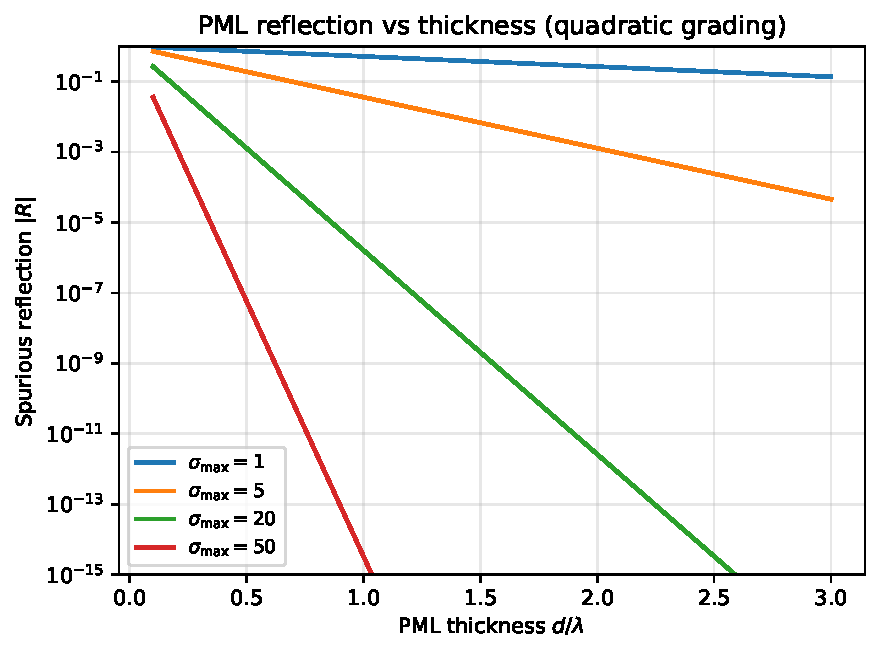
\includegraphics[width=0.68\linewidth]{figures/fig_f17_pml_reflection.pdf}
 \caption{Spurious PML reflection for a polynomial absorption profile.
 For quadratic grading the approximate reflection decreases
 exponentially with both PML thickness $d_{\mathrm{PML}}/\lambda$ and
 maximum absorption $\sigma_{\max}$. The plot explains why PML
 convergence checks must vary both parameters: too thin or too weak a
 PML produces artificial resonances, while excessively strong absorption
 can introduce discretization error.}
 \label{fig:pml-reflection}
\end{figure}

\subsection{Challenges of non-Hermiticity}
\label{ssec:fem-challenges}

\begin{enumerate}
 \item \textbf{Non-symmetric matrices.} When $\epsr$ is complex, the
 matrices $\mathbf{A}$ and $\mathbf{B}$ are no longer Hermitian
 (though they may remain complex symmetric for reciprocal media).
 Standard Hermitian eigensolvers (Lanczos, LOBPCG) cannot be used;
 Arnoldi-type solvers or contour-integral methods are
 required~\cite{wu2026rigorous}.

 \item \textbf{Spurious PML eigenvalues.} PML modes---artifacts of the
 truncated absorbing layer---appear alongside the physical QNMs in
 the computed spectrum. They must be identified and filtered
 (Section~\ref{sec:pml-validation}).

 \item \textbf{Eigenvalue conditioning.} Near an exceptional point,
 eigenvalues are extremely sensitive to perturbations
 ($\epsilon^{1/2}$ scaling, Section~\ref{sec:ep2}). Fine meshes and
 high-order elements are needed to resolve the EP accurately.

 \item \textbf{Frequency-dependent materials.} When $\epsr(\omega)$
 is dispersive (e.g., Drude or Lorentz), the eigenvalue problem
 becomes nonlinear in $\omega$. Linearization through auxiliary
 fields or polynomial eigenproblem formulations is needed
 (Section~\ref{sec:dispersive-evp}).

 \item \textbf{Biorthogonal post-processing.} Modal overlaps, Purcell
 factors, and coupling coefficients require the adjoint eigenvectors
 (Section~\ref{sec:qnm-adjoint}), which must be computed from the
 transposed problem~\cite{vial2014quasimodal}.

 \item \textbf{Mesh refinement rule.} For standard second-order
 N\'ed\'elec elements, the mesh size should satisfy
 $h < \lambda/(10\,n_{\max})$, where $n_{\max}$ is the largest
 refractive index in the computational domain. Near metallic
 or high-index interfaces, local refinement to $h \sim \lambda/30$
 is typically needed to resolve evanescent tails and surface currents.
 For high-order elements (order $p \ge 3$), the global mesh
 constraint can be relaxed to $h < \lambda/(5\,n_{\max})$, but local
 refinement at material discontinuities remains essential. A useful
 convergence test is to verify that the QNM eigenfrequency changes by
 less than $0.1\%$ when the mesh is uniformly refined by a factor of
 two.
\end{enumerate}

\begin{figure}[t]
 \centering
 
\includegraphics[width=0.62\linewidth]{fig_f17_fem_convergence.pdf}
 \caption{Convergence of a QNM eigenfrequency with mesh refinement
 for linear ($p = 1$, blue circles) and quadratic ($p = 2$, red
 squares) N\'ed\'elec edge elements. The relative error scales as
 $N^{-2}$ and $N^{-4}$ respectively, where $N$ is the number of
 mesh elements. This schematic illustrates the expected algebraic
 convergence rates; actual rates depend on the resonator geometry,
 material contrast, and PML parameters. Quadratic elements reach
 substantially smaller errors with approximately $10^4$ elements, while
 linear elements require substantially finer meshes for the same target
 accuracy.}
 \label{fig:fem-convergence}
\end{figure}


%% ================================================================
\section{QNM extraction and normalization}
\label{sec:qnm-extraction}

\subsection{Shift-and-invert Arnoldi}
\label{ssec:arnoldi}

The most common approach to extracting a few QNMs near a target
frequency $\omega_0$ is the shift-and-invert Arnoldi method. The
generalized eigenvalue problem~\eqref{eq:fem-gep} is transformed to
\begin{equation}
 (\mathbf{A} - \omega_0^2\,\mathbf{B})^{-1}\,\mathbf{B}\,\mathbf{x}
 = \mu\,\mathbf{x},
 \qquad \mu = \frac{1}{\omtil^2 - \omega_0^2},
 \label{eq:shift-invert}
\end{equation}
and the Arnoldi iteration is applied to the transformed operator.
Eigenvalues $\omtil$ closest to $\omega_0$ correspond to the largest
$|\mu|$ and converge first.

For non-Hermitian problems, the Arnoldi algorithm (rather than
Lanczos) must be used because the operator is not self-adjoint. The
resulting eigenvalues are generally complex, and the left and right
Arnoldi vectors differ.

\subsection{Pole-search methods}
\label{ssec:pole-search}

An alternative to matrix eigensolvers is to search for poles of a
scalar response function (e.g., a scattering coefficient or an
extinction cross-section) directly in the complex $\omega$
plane~\cite{wu2026rigorous}. Starting from an initial guess $\omega^{(0)}$
near a resonance, one applies Newton iteration to a function that
vanishes at the pole, such as the inverse of the response:
\begin{equation}
 \omega^{(n+1)} = \omega^{(n)}
 - \frac{q(\omega^{(n)})}{q'(\omega^{(n)})},
 \label{eq:pole-search-newton}
\end{equation}
where $q(\omega)$ is the inverse-response function and $q'$ is its derivative
(computed by a finite difference in $\omega$ or by adjoint sensitivity~\cite{v2024exact,ren2021quasinormal}).
This Newton-type iteration converges quadratically and typically
requires fewer than 10 full-wave solves per
pole~\cite{wu2026rigorous}.

The pole-search approach has the advantage that each iteration uses a
driven frequency-domain FEM solve at a complex frequency, with material
dispersion analytically continued as needed, avoiding the need to solve
a large generalized eigenvalue problem~\cite{wu2026rigorous,berlin2024poles}. It is the basis of the MAN (Modal Analysis
of Nanoresonators) software package~\cite{wu2026rigorous}.

\subsection{QNM normalization in practice}
\label{ssec:normalization-practice}

Once a QNM eigenfrequency $\omtil_n$ and its field profile
$\tilde{\EE}_n$ are known, the normalization factor
(Section~\ref{sec:qnm-normalization}) must be computed. In a PML-based
FEM framework, the unconjugated volume integral over the computational
domain (including the PML) provides a well-defined normalization:
\begin{equation}
 N_n = \int_{\Omega + \mathrm{PML}}
 \left[\tilde{\EE}_n \cdot \pdv{(\omega\epsr)}{\omega}\bigg|_{\omtil_n}
 \tilde{\EE}_n
 - \tilde{\HH}_n \cdot \pdv{(\omega\mur)}{\omega}\bigg|_{\omtil_n}
 \tilde{\HH}_n\right]\dd V,
 \label{eq:normalization-pml}
\end{equation}
where the derivatives account for material dispersion; for a
nonmagnetic nondispersive background, the magnetic term reduces to
$-\tilde{\HH}_n\cdot\tilde{\HH}_n$ up to the unit convention used in the
Maxwell operator~\cite{wu2026rigorous}. The normalization is complex.
After choosing a normalization convention, the QNM mode volume at a
dipole position $\rr_0$ is proportional to
$1/[\epsr(\rr_0)\tilde{\EE}_n(\rr_0)\cdot\tilde{\EE}_n(\rr_0)]$ and is
therefore generally complex.

\begin{remark}
The historical difficulty with QNM normalization---which delayed the
development of practical QNM methods by
decades~\cite{wu2026rigorous}---is now well understood for many
PML-regularized and dispersive formulations. The key insight
is that the unconjugated inner product, combined with the PML
regularization, yields a normalization that is both mathematically
rigorous and numerically stable.
\end{remark}


%% ================================================================
\section{PML validation and spurious-mode filtering}
\label{sec:pml-validation}

The PML converts the continuous radiation spectrum into a discrete set
of PML modes, which contaminate the computed eigenvalue spectrum.
Distinguishing physical QNMs from PML artifacts is essential.

\subsection{PML parameter variation}
\label{ssec:pml-variation}

The most reliable test is to vary the PML parameters (thickness
$d_{\mathrm{PML}}$, absorption strength $\sigma_{\max}$, polynomial
order $p$) and track which eigenvalues are stable:
\begin{itemize}
 \item \textbf{Physical QNMs}: their eigenfrequencies $\omtil_n$ are
 independent of PML parameters (up to exponentially small
 corrections that decrease with PML thickness).
 \item \textbf{PML modes}: their eigenfrequencies depend strongly on
 the PML parameters and move in the complex plane as $d_{\mathrm{PML}}$
 or $\sigma_{\max}$ is changed.
\end{itemize}

\begin{figure}[t]
 \centering
 
\includegraphics[width=0.95\textwidth]{fig_f17_pml_convergence.pdf}
 \caption{PML validation by parameter variation in the complex-frequency
 plane. A physical quasinormal-mode pole remains nearly fixed as the PML
 absorption strength is varied and approaches a limiting pole, whereas
 modes associated with the discretized radiation continuum move
 appreciably. This stability check is a practical way to separate
 physical resonances from PML-dominated branches.}
 \label{fig:pml-convergence}
\end{figure}

\subsection{Mode-ratio criterion}
\label{ssec:mode-ratio}

An alternative criterion uses the \emph{mode ratio}:
\begin{equation}
 \mathrm{MR}_n = \frac{\int_{\Omega_{\mathrm{phys}}}
 |\tilde{\EE}_n|^2\;\dd V}
 {\int_{\Omega_{\mathrm{phys}} + \mathrm{PML}}
 |\tilde{\EE}_n|^2\;\dd V},
 \label{eq:mode-ratio}
\end{equation}
where $\Omega_{\mathrm{phys}}$ is the physical domain (excluding the
PML). Physical QNMs have most of their energy in the physical domain
($\mathrm{MR}_n$ close to 1 for high-$\Qfac$ modes), while PML modes
are concentrated in the absorbing layer
($\mathrm{MR}_n \ll 1$)~\cite{wu2026rigorous}.

\begin{figure}[t]
 \centering
 
\includegraphics[width=0.95\textwidth]{fig_f17_pml_mode_ratio.pdf}
 \caption{The mode-ratio criterion separates physical resonances from PML-dominated modes. In this reproducible validation example, the physical QNM has mean mode ratio near $0.946$, while the synthetic PML-mode cloud has mean mode ratio near $0.109$. The plot illustrates why a computed complex eigenfrequency should not be accepted as a physical resonance unless both its PML stability and its field localization have been checked.}
 \label{fig:pml-mode-ratio}
\end{figure}

\begin{booknote}[PML modes are not errors]
PML modes are not numerical artifacts in the sense of discretization
errors---they are the discretized representation of the continuous
radiation spectrum. They are \emph{necessary} for completeness of the
modal expansion (Section~\ref{sec:qnm-completeness}) but should not be
confused with physical resonances. The PML validation step is not about
removing errors but about classifying different parts of the spectrum.
\end{booknote}


%% ================================================================
\section{Contour-integral eigensolvers}
\label{sec:contour-eigensolvers}

For problems where many QNMs are needed in a specified frequency range,
or where the eigenvalues are densely clustered, contour-integral
eigensolvers offer a systematic approach.

\subsection{The principle}
\label{ssec:contour-principle}

Contour-integral methods exploit Cauchy's integral formula to project
onto the eigenspace associated with eigenvalues inside a closed contour
$\mathcal{C}$ in the complex $\omega$ plane. For a meromorphic
matrix-valued function $\mathbf{M}(\omega)$, the contour integrals
\begin{equation}
 \mathbf{S}_p = \frac{1}{2\pi i}\oint_{\mathcal{C}}
 \omega^p\,\mathbf{M}(\omega)^{-1}\,\mathbf{R}\;\dd\omega,
 \qquad p = 0, 1, 2, \ldots
 \label{eq:contour-moments}
\end{equation}
(where $\mathbf{R}$ is a random probe matrix) yield generalized moment
matrices from which the eigenvalues and eigenvectors inside
$\mathcal{C}$ can be extracted by solving a small projected
eigenproblem~\cite{berlin2024poles}.

\subsection{Beyn's algorithm}
\label{ssec:beyn}

Beyn's algorithm~\cite{berlin2024poles,cui2024roadmap} is the most
widely used contour-integral eigensolver for non-Hermitian photonic
problems. Its appeal lies in simplicity: it requires only the ability
to solve $\mathbf{M}(\omega_q)\,\mathbf{y} = \mathbf{r}$ at a set of
complex frequencies $\omega_q$ on the contour, a capability that any
frequency-domain FEM code already provides.

\paragraph{Step 1: Moment computation.}
Choose a contour $\mathcal{C}$ in the complex $\omega$ plane that
encloses the eigenvalues of interest, and a random probe matrix
$\mathbf{R} \in \mathbb{C}^{N \times L}$ with $L$ columns (typically
$L \ge 2k$, where $k$ is an upper bound on the number of enclosed
eigenvalues). Approximate the contour integrals~\eqref{eq:contour-moments}
by numerical quadrature with $N_q$ points:
\begin{equation}
 \mathbf{S}_p \approx \frac{1}{2\pi i}\sum_{q=1}^{N_q}
 w_q\,\omega_q^p\,\mathbf{M}(\omega_q)^{-1}\,\mathbf{R},
 \qquad p = 0, 1,
 \label{eq:beyn-quadrature}
\end{equation}
where $w_q$ and $\omega_q$ are quadrature weights and nodes (typically
the trapezoidal rule on a circle or ellipse, which converges
exponentially for analytic integrands). Each quadrature point requires
one sparse linear solve of the FEM system at the complex frequency
$\omega_q$; these solves are embarrassingly parallel.

\paragraph{Step 2: Rank-revealing SVD.}
Compute the singular value decomposition
$\mathbf{S}_0 = \mathbf{U}\,\boldsymbol{\Sigma}\,\mathbf{V}^H$.
The number of eigenvalues $k$ inside $\mathcal{C}$ is determined by the
number of singular values above a threshold $\sigma_j > \epsilon\,\sigma_1$.
The choice of threshold $\epsilon$ is the main user decision:
$\epsilon \sim 10^{-8}$ is typical. If all singular values are below
the threshold, the contour contains no eigenvalues and the algorithm
terminates.

\paragraph{Step 3: Reduced eigenproblem.}
Truncate to the first $k$ singular values and form the $k \times k$
projected matrix
\begin{equation}
 \mathbf{B}_{\mathrm{Beyn}}
 = \mathbf{U}_k^H\,\mathbf{S}_1\,\mathbf{V}_k\,
 \boldsymbol{\Sigma}_k^{-1}.
 \label{eq:beyn-reduced}
\end{equation}
The eigenvalues of $\mathbf{B}_{\mathrm{Beyn}}$ are the QNM complex
frequencies inside $\mathcal{C}$. If
$\mathbf{B}_{\mathrm{Beyn}}\mathbf{v}_j=\omega_j\mathbf{v}_j$, the
corresponding approximate eigenvector of the original problem is
recovered as
\begin{equation}
 \mathbf{x}_j =
 \mathbf{S}_0\,\mathbf{V}_k\,\boldsymbol{\Sigma}_k^{-1}\mathbf{v}_j .
 \label{eq:beyn-eigenvector}
\end{equation}
The computational cost is dominated by the $N_q$ sparse linear solves;
the SVD and reduced eigenproblem are negligible.

\paragraph{Convergence.}
The quadrature error decreases exponentially with $N_q$ for smooth
contours enclosing well-separated eigenvalues. However, when an
eigenvalue sits close to $\mathcal{C}$, the integrand becomes
near-singular and convergence slows dramatically. The practical remedy
is to use adaptive contours that keep a minimum distance from all
eigenvalues, or to use rational quadrature rules that concentrate nodes
near potential singularities. A typical rule of thumb for photonic
applications is $N_q \ge 4k + 10$, where $k$ is the estimated number
of enclosed eigenvalues.

\paragraph{Validation.}
After extracting the eigenvalues, each should be validated by computing
the residual $\|\mathbf{M}(\omega_j)\mathbf{x}_j\|/\|\mathbf{x}_j\|$.
Spurious eigenvalues from PML artifacts or insufficient quadrature
typically have residuals many orders of magnitude larger than the
physical QNMs. This residual check, combined with the PML-eigenvalue
filtering of Section~\ref{sec:pml-validation}, provides a robust
workflow for extracting clean QNM spectra from complex photonic
structures.

\subsection{FEAST algorithm}
\label{ssec:feast}

The FEAST algorithm~\cite{wu2026rigorous,opg2023dispersive} is a
contour-integral eigensolver originally developed for Hermitian
problems and later extended to non-Hermitian and polynomial eigenvalue
problems~\cite{jgopalakrishnan2022computing}. While Beyn's algorithm
extracts eigenvalues from moments $\mathbf{S}_0$ and $\mathbf{S}_1$
by solving a linearized pencil, FEAST instead uses the contour
integral as a spectral projector and iterates the subspace to
self-consistency.

The FEAST iteration proceeds as follows. Given an initial subspace
$\mathbf{Q}^{(0)} \in \mathbb{C}^{N \times m}$ (where $m \ge k$),
compute the filtered subspace
\begin{equation}
 \mathbf{Q}^{(i+1)} = \frac{1}{2\pi i}\oint_{\mathcal{C}}
 \mathbf{M}(\omega)^{-1}\,\mathbf{Q}^{(i)}\;\dd\omega,
 \label{eq:feast-iteration}
\end{equation}
then solve the projected eigenproblem in the filtered subspace. The
iteration converges when the Ritz values stabilize. For Hermitian
problems with a well-separated interval and accurate quadrature, FEAST
has a robust convergence theory; for non-Hermitian problems, convergence
depends more sensitively on eigenvalue separation, non-normality, and
the conditioning of the spectral projector.

For frequency-dependent PML, the Maxwell eigenproblem becomes a
polynomial eigenvalue problem:
\begin{equation}
 \left(\mathbf{A}_0 + \omega\,\mathbf{A}_1
 + \omega^2\,\mathbf{A}_2
 + \omega^3\,\mathbf{A}_3\right)\mathbf{x} = 0,
 \label{eq:polynomial-evp}
\end{equation}
where the cubic term arises from the frequency dependence of the PML
stretching factor $s_\alpha(\omega)$. FEAST handles this by
linearization into a block companion-matrix problem and contour
integration over the resulting linear
pencil~\cite{jgopalakrishnan2022computing}. The linearization
increases the matrix dimension by a factor equal to the polynomial
degree, but the contour integral projects back onto the physical
subspace, keeping the effective problem size manageable.

\paragraph{Beyn vs.\ FEAST.}
Both algorithms share the same computational bottleneck---sparse linear
solves at complex frequencies---and both converge exponentially with
the number of quadrature points. The main practical difference is that
FEAST is iterative and can refine the subspace over multiple sweeps,
which is advantageous when the initial subspace is poor or when very
high accuracy is needed. Beyn's algorithm is non-iterative and
extracts all eigenvalues in a single pass, making it simpler to
implement but potentially less accurate for eigenvalues near the
contour. For photonic applications, both algorithms have been
demonstrated to extract QNM spectra with residuals below
$10^{-10}$~\cite{wu2026rigorous}.

\subsection{Poles and zeros simultaneously}
\label{ssec:poles-zeros}

The same contour-integral machinery can compute both the
\emph{poles} (QNMs) and \emph{zeros} (CPA conditions) of a scalar
scattering coefficient $q(\omega)$ from the same set of contour
integrals~\cite{berlin2024poles}. The poles of $q$ and the poles of
$1/q$ are extracted simultaneously using Hankel matrices built from the
contour moments of $q(\omega)$ and $q(\omega)^{-1}$. This gives a
local pole-zero map of the scattering response inside the chosen contour,
connecting directly to the framework of
Chapter~\ref{ch:poles-zeros}.


%% ================================================================
\section{Dispersive materials and nonlinear eigenproblems}
\label{sec:dispersive-evp}

When $\epsr(\omega)$ is frequency-dependent (Section~\ref{sec:complex-eps}),
the eigenvalue problem~\eqref{eq:fem-gep} becomes nonlinear in $\omega$:
$\mathbf{A}(\omega)\,\mathbf{x} = 0$. Several strategies exist.

\subsection{Auxiliary-field linearization}
\label{ssec:aux-linearization}

For Lorentz-type dispersion~\eqref{eq:lorentz-eps}, the auxiliary-field
technique of Section~\ref{sec:auxiliary-fields} introduces polarization
currents as additional unknowns, converting the nonlinear eigenproblem
into a linear (but larger) generalized eigenproblem:
\begin{equation}
 \begin{pmatrix}
 \mathbf{A}_{\mathrm{curl}} & \mathbf{C} \\
 \mathbf{D} & \mathbf{A}_{\mathrm{osc}}
 \end{pmatrix}
 \begin{pmatrix} \mathbf{x}_E \\ \mathbf{x}_P \end{pmatrix}
 = \omega
 \begin{pmatrix}
 \mathbf{B}_E & 0 \\
 0 & \mathbf{B}_P
 \end{pmatrix}
 \begin{pmatrix} \mathbf{x}_E \\ \mathbf{x}_P \end{pmatrix},
 \label{eq:aux-linearized}
\end{equation}
where $\mathbf{x}_E$ represents the electric field DOFs and
$\mathbf{x}_P$ the auxiliary polarization DOFs. This linearized system
can be solved by standard non-Hermitian eigensolvers.

\subsection{Polynomial eigenproblem}
\label{ssec:polynomial-evp}

For more general dispersion models (Drude, multi-pole Lorentz, or
frequency-dependent PML), the eigenproblem is polynomial in $\omega$
with degree $d > 2$~\cite{jgopalakrishnan2022computing}. Linearization
by companion-matrix embedding converts a degree-$d$ polynomial
eigenproblem of size $N$ into a linear eigenproblem of size $dN$,
which can be impractical for large FEM discretizations.

Contour-integral eigensolvers (Section~\ref{sec:contour-eigensolvers})
avoid explicit linearization by working directly with the nonlinear
$\mathbf{A}(\omega)$, evaluating it at quadrature points on the contour.
This is often more efficient than linearization when only a few
eigenvalues are needed.

\subsection{Convergence caveats}
\label{ssec:convergence-caveats}

For dispersive PML, Gopalakrishnan et al.\ showed that computed loss
values can be off by orders of magnitude if the FEM mesh and polynomial
order are not in the asymptotic convergence regime: careful $h$- and
$p$-refinement studies are essential before trusting the imaginary part
of $\omtil$~\cite{jgopalakrishnan2022computing}. This is a pitfall
that is often overlooked in the photonics literature, where convergence
is checked against $\Re\omtil$ but not $\Im\omtil$.


%% ================================================================
\section{Plane-wave expansion for complex bands}
\label{sec:pwe-complex}

The plane-wave expansion (PWE) method of Section~\ref{sec:unit-cell}
extends naturally to complex $\epsr(\rr)$: the Fourier
coefficients $\hat{\eps}_{\GG}$ become complex, and the eigenvalue
matrix is no longer Hermitian. The resulting complex band structure
$\omega_n(\kk)$ is computed by standard dense or iterative non-Hermitian
eigensolvers (LAPACK \texttt{zgeev} for small problems, Arnoldi for
large ones).

\subsection{Computing topological invariants}
\label{ssec:pwe-topology}

From the complex Bloch eigenstates on a grid of $\kk$-points, the
Berry curvature, Chern number, and spectral winding number can be
computed using the discretized formulas of
Section~\ref{sec:berry-numerical}. For the non-Bloch invariants
(Section~\ref{sec:non-bloch-invariants}), the PWE must be performed on
the appropriate complex wave-vector contour rather than on the real BZ.
For tight-binding or transfer-matrix reductions this is the GBZ contour
obtained from the characteristic roots. For a continuum Maxwell PWE
calculation, the analogous computation is a complex-$\kk$ band problem
and must be validated against the finite-structure spectrum.

\subsection{Non-Bloch PWE}
\label{ssec:non-bloch-pwe}

Computing the non-Bloch band structure requires evaluating
$\omega_n(\beta)$ for complex $\beta = e^{ik}$ on the GBZ contour
(Section~\ref{sec:gbz}). In a lattice model this amounts to replacing
$e^{ik}$ by the complex number $\beta$ in the hopping phases. In a
continuum PWE calculation, it is better viewed as solving the Maxwell
operator at complex Bloch wave vector $k+i\kappa$; the Fourier basis is
still periodic in the unit cell, but the full field carries an
exponential envelope across cells. The resulting contour is not
automatically the physical GBZ and should be checked by comparing the
predicted non-Bloch spectrum with open-boundary simulations.


%% ================================================================
\section{FDTD with gain and loss}
\label{sec:fdtd}

The finite-difference time-domain (FDTD) method propagates Maxwell's
equations directly in time on a spatial grid. For non-Hermitian systems,
the complex permittivity introduces gain or loss at each time step:
\begin{equation}
 \pdv{\DD}{t} = \curl\HH - \sigma\,\EE,
 \label{eq:fdtd-ampere}
\end{equation}
where $\sigma(\rr)$ is the conductivity (positive for loss, negative
for gain in a linearized model).

\subsection{Stability and gain saturation}
\label{ssec:fdtd-stability}

Gain media can make the FDTD simulation unstable: the field grows
exponentially and eventually overflows. Two remedies are common:
\begin{itemize}
 \item \textbf{Gain saturation models:} replace the linear gain
 $\sigma < 0$ with a nonlinear model
 $\sigma_{\mathrm{eff}} = \sigma_0 / (1 + |\EE|^2/E_{\mathrm{sat}}^2)$
 that clamps the amplification at high field intensities.
 \item \textbf{Windowed time analysis:} run the simulation for a
 limited time before overflow and extract QNM frequencies from the
 ring-down signal.
\end{itemize}

\subsection{Extracting QNM frequencies from time series}
\label{ssec:harmonic-inversion}

The complex QNM frequencies can be extracted from FDTD time series
using harmonic inversion: the decaying signal $f(t) = \sum_n A_n
e^{-i\omtil_n t}$ is fitted to a sum of complex exponentials using
Pad\'e approximation, the filter diagonalization method, or Prony's
method. The accuracy of the extracted $\omtil_n$ depends on the
signal-to-noise ratio and the spectral separation of the modes.


%% ================================================================
\section{Specialized algorithms}
\label{sec:specialized}

\subsection{EP tracking}
\label{ssec:ep-tracking}

Finding exceptional points in parameter space requires tracking the
coalescence of eigenvalues. Efficient algorithms include:
\begin{itemize}
 \item \textbf{Newton iteration on the discriminant:} solve
 $\Delta(\mathbf{p}) = 0$ where $\Delta$ is the discriminant of
 the characteristic polynomial and $\mathbf{p}$ are the system
 parameters. For a $2\times 2$ subsystem,
 $\Delta = (\omtil_+ - \omtil_-)^2$; the EP is located where
 $\Delta = 0$.
 \item \textbf{Encircling methods:} sweep parameters along a closed
 loop and check for eigenvalue exchange (Section~\ref{sec:encircling}),
 which signals an enclosed EP. This method is robust but
 requires many eigenvalue evaluations.
 \item \textbf{Perturbation theory:} expand the eigenvalue splitting
 around a known near-EP configuration to predict the EP location
 to first order. This is fast but may fail far from the EP.
\end{itemize}

Near higher-order EPs (EP$_3$, EP$_4$), the tracking problem is
more difficult because more parameters must be tuned simultaneously
and the eigenvalue sensitivity is extreme.

\subsection{GBZ computation}
\label{ssec:gbz-computation}

Computing the generalized Brillouin zone (Section~\ref{sec:gbz}) requires
solving the auxiliary polynomial~\eqref{eq:gbz-condition} at each energy.
For a two-band model, this is a quartic equation in $\beta$; for
multi-band models, the degree increases accordingly. Practical
approaches include:
\begin{itemize}
 \item \textbf{Companion-matrix eigensolvers:} convert the polynomial
 $P(\beta, \omega) = 0$ to a companion-matrix eigenproblem and solve
 for all roots at each $\omega$.
 \item \textbf{Root tracking:} start from a known root at one
 $\omega$ and track it continuously as $\omega$ varies, using
 Newton's method with the previous root as the initial guess.
 \item \textbf{Contour-integral root finding:} apply the
 contour-integral technique of
 Section~\ref{sec:contour-eigensolvers} to the polynomial
 $P(\beta, \omega)$, treating $\beta$ as the eigenvalue.
\end{itemize}


%% ================================================================
\section{Practical guidelines}
\label{sec:numerical-guidelines}

\begin{enumerate}
 \item \textbf{PML validation is mandatory.} Always verify QNM
 eigenvalues against PML parameter variation
 (Section~\ref{sec:pml-validation}). Never trust a QNM frequency
 obtained with a single PML configuration.

 \item \textbf{Convergence of $\Im\omtil$ is harder than $\Re\omtil$.}
 The imaginary part of the eigenfrequency (the decay rate) converges
 more slowly with mesh refinement than the real part. Always check
 both~\cite{jgopalakrishnan2022computing}.

 \item \textbf{EP-sensitive problems need special care.} Near an EP,
 use high-order elements, fine $\kk$-grids, and verify with
 independent methods. The $\sqrt{\epsilon}$ eigenvalue splitting
 amplifies discretization errors.

 \item \textbf{Non-Bloch invariants require accurate GBZ.} Errors
 in the GBZ contour propagate directly to the non-Bloch topological
 invariant. Use high-precision root finding and verify by comparing
 PBC and OBC spectra.

 \item \textbf{FDTD with gain requires a stability strategy.} Always
 include a saturation model or truncate the simulation before
 numerical overflow. Harmonic inversion from a short windowed
 signal is often more reliable than a long, unstable run.

 \item \textbf{Cross-validate between methods.} Compare FEM and PWE,
 or FEM and FDTD, whenever possible. Agreement between independent
 methods is the strongest evidence for correctness in non-Hermitian
 problems where physical intuition may mislead.

 \item \textbf{Use biorthogonal post-processing.} For modal
 quantities (Purcell factors, coupling coefficients, perturbation
 theory), always use the biorthogonal normalization of
 Section~\ref{sec:qnm-normalization}, not the Hermitian norm.
\end{enumerate}

\begin{takeaway}[Non-Hermiticity changes the numerical landscape]
Standard photonic simulation tools---FEM, PWE, FDTD---remain the
workhorses, but non-Hermiticity introduces new challenges: non-symmetric
matrices, spurious PML modes, EP sensitivity, gain instability,
dispersive nonlinear eigenproblems, and the need for biorthogonal
post-processing and GBZ-based invariant computation. The validation
protocol---PML variation, mode-ratio filtering, convergence checks on
both $\Re\omtil$ and $\Im\omtil$, cross-method comparison---is not
optional: it is the price of doing reliable numerical non-Hermitian
photonics.
\end{takeaway}
